
\section{Abstract}

In many species, spatial navigation is supported by a network of ``place cells'' that exhibit increased firing whenever an animal is in a certain region of an environment. Does this neural representation of location form part of the spatiotemporal context into which episodic memories are encoded? We recorded medial temporal lobe neuronal activity as neurosurgical patients performed a hybrid spatial and episodic memory task.  We identified place-responsive cells active during virtual navigation and then asked whether the same cells activated during the subsequent recall of navigation-related memories without actual navigation. Place-responsive cell activity was reinstated during episodic memory retrieval. Neuronal firing during the retrieval of each memory was  similar to the activity that represented the locations in the environment  where the memory was initially encoded.


\section{Introduction, Results, and Discussion}
When one encounters an old friend and remembers the time they last met, often the place of meeting and surrounding circumstances come to mind. This is the hallmark of episodic memory---the capacity to store and later retrieve memories that are bound to a particular place and time \cite{Tulv83}.  Theories of episodic memory posit that the brain supports this ability by continually maintaining an updated representation of the current spatiotemporal context, which is a neural representation of space, time, and other aspects of one's current cognitive milieu \cite{PolyKaha08}.  When the brain forms a new episodic memory, these theories predict that the content of the experience becomes associated with the current spatial and temporal context.  When the memory is retrieved, this prior context is partially reinstated, focusing one's thoughts on time and place of the remembered episode. This reinstatement not only provides the phenomenological experience of remembering, but it also helps to cue other memories experienced within the same or related contexts.

Although it is well established that the hippocampus and surrounding medial-temporal-lobe (MTL) structures play a central role in the formation and retrieval of context-mediated memories \cite{ScovMiln57,Eich04,Dava06}, we know far less about how these memory processes manifest in the activities of individual MTL neurons.  Much of what is known about the neural coding properties of hippocampal and MTL neurons comes from studies of rodent spatial navigation, where individual neurons respond preferentially at specific  locations within a given contextually-defined spatial environment  \cite{OKeeNade78,McNaEtal06}.  Similar neuronal responses have also been identified in the human hippocampus during virtual spatial navigation \cite{EkstEtal03,JacoEtal10}.  The context dependent firing of these neurons \cite{MullKubi87,LeutEtal05} and their dependence on the animal's goal state or past history of experienced cues \cite{WoodEtal00,FerbShap03} has led some to speculate that the neural representation of space in the hippocampus is  part of a broader network of neurons that encode episodic memories more generally \cite{EichEtal99,Buzs05,HowaEtal05,BuzsMose13}.  This hypothesis suggests that the same neural structures and computations that enable the learning of a spatial layout via place cell activity also facilitate encoding episodic memories. However, according to a prominent alternative account, the spatial coding functions of the hippocampus are part of a context module that operates independently of the computations that encode the content of a memory \cite{DavaEtal03,HargEtal05}.

\begin{figure}
  \begin{center} \centering
    \includegraphics[width=.8\textwidth]{./tex/dboy/figs/fig1}
  \caption[Delivery Person task design]{The behavioral task. \textbf{A.} Overhead map of the virtual environment. Red rectangles indicate store locations, and blue squares indicate locations of non-store buildings. Green areas indicate grass and trees, and the small dark blue, brown, and yellow boxes represent mailboxes, benches, and street lights. \textbf{B.} An example storefront that a subject might encounter. \textbf{C.} The presentation of an item (a zucchini) upon arrival at the target store (bakery). \textbf{D.} The initiation of the recall period, as indicated by a black screen with asterisks.}
\label{fig:dboy_town}
\end{center}
\end{figure}

We designed a virtual-reality memory game in which subjects played the role of a delivery person, driving through a virtual town and delivering objects to stores.  Our subjects were patients with drug resistant epilepsy who were implanted with depth electrodes to localize the focus of their seizures and to map cognitive function in surrounding healthy tissue. In an initial phase of the game, subjects explored the town using a computer controller to navigate from store to store as they attempted to learn the layout of the environment illustrated in Fig.~\ref{fig:dboy_town}A.  After this initial familiarization phase, during which subjects visited each store twice, they began a series of ``delivery days''.  On each delivery day, subjects were instructed to travel from store to store, visiting 13 randomly chosen stores (of the 16 total) in a randomly determined order.  Upon their arrival at each store, they were presented with an object (either visually for 2 sec for subjects 1 - 5 or aurally for subjects 6 - 7).  Upon arrival at the final (13th) store, no item was presented. Instead, the screen went black and subjects were prompted to vocally recall as many of the 12 delivered objects as they could remember in any order (subjects recalled 5.2 objects, on average).  After being given 90 seconds for free recall, subjects could advance to a new delivery day, in which they would deliver a unique but randomly determined set of objects to a random sequence of 13 stores and then attempt to recall the new set of objects. Consistent with prior work \cite{MillEtal12a}, subjects exhibited a significant ($p=.008$) tendency to consecutively recall objects delivered to more spatially proximate locations (see supplementary  text).

% \section{Results}
% 
We first sought to identify patterns of neuronal activity that represented subjects' location within the virtual town. We identified place-responsive cells as the neurons that exhibited significantly increased firing at a particular location in the virtual environment. Fig.~\ref{fig:place_ex}A depicts the activity of one example place-responsive cell, which increased its firing rate when the subject was positioned at a location on the left side of the virtual environment and facing north.  The majority of the identified place-responsive cells were direction dependent (72\%) and did not exhibit significant place fields when direction of traversal was not taken into account.  This is similar to prior findings of directionally oriented place cells in environments with clearly defined routes, in contrast to open environments, where omnidirectional place cells are prevalent \cite{MullEtal94,EkstEtal03}.  These directionally-oriented place cells were not generally responsive to place-invariant view information. Fig.~\ref{fig:place_ex}B shows the firing rate of a place-responsive cell from the entorhinal cortex, which activated at a location in the south part of the environment during eastward movements.  In total, we identified 95 place-responsive cells, comprising 25.6\% of all observed neurons. There were significant numbers of place-responsive cells in the hippocampus, entorhinal cortex, amygdala, and in anterior MTL regions of ambiguous localization (binomial test with $p<0.01$ for each region, Fig.~\ref{fig:place_ex}C, Tables \ref{tab:counts} and \ref{tab:counts2}).

\begin{figure}
\centering
    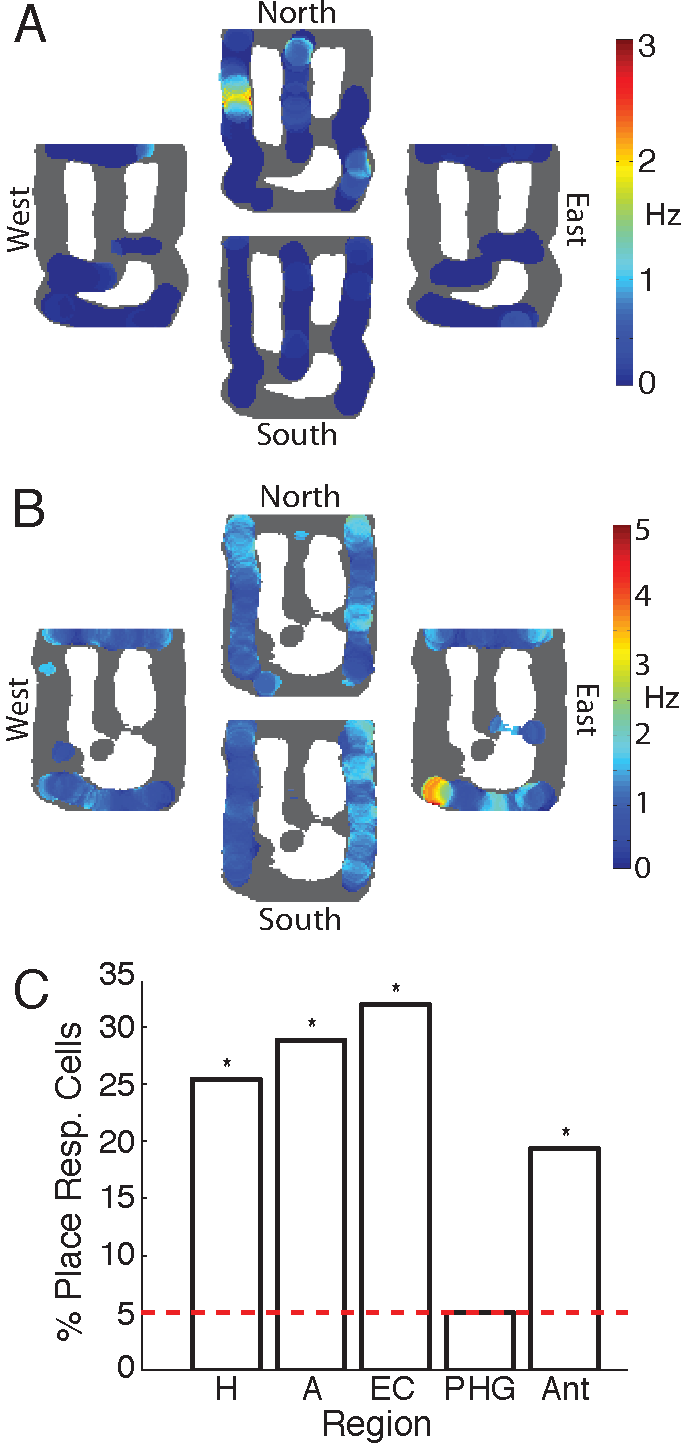
\includegraphics[width=.5\textwidth]{./tex/dboy/figs/fig2}
  \caption[Place-responsive cells]{Place-responsive cells.  \textbf{A}. Firing rate map for a cell responsive to northward traversals located in Subject 6's hippocampus, shown separately for each cardinal direction. Grey represents all areas traversed by the subject, regardless of direction of travel. \textbf{B.} A cell responsive to eastward traversals recorded from Subject 1's entorhinal cortex. \textbf{C.} The regional distribution of place-responsive cells in the entire dataset of 371 single units (H: hippocampus, A: amygdala, EC: entorhinal cortex, PHG: parahippocampal gyrus, Ant: anterior MTL, not otherwise specified).  The red line indicates the false positive rate of 5\%.}
\label{fig:place_ex}
\end{figure}

To determine whether spontaneous retrieval of items during free recall reinstated the spatial context associated with the item's encoding, we calculated the neural similarity between ensemble place-responsive cell activity during navigation and during item retrieval (see Fig.~\ref{fig:methods} for further details).  We partitioned the environment into three regions for each recalled item: regions close to the delivery location, regions of intermediate distance, and regions that were far from the delivery location.  We then asked whether the ensemble place-cell activity at the time of retrieval was more similar to navigational epochs that were closer to the delivery location.  A high degree of similarity would indicate the reinstatement of the spatial context associated with the item.  To protect against potential confounding between object and spatial context, we excluded navigational epochs surrounding the delivery of an object.  

We found significant spatial context reinstatement surrounding the time of item vocalization (timecourse illustrated in Fig.~\ref{fig:reinstate}A). The level of neural similarity between recall activity and navigation activity was ordered such that areas of the environment near  an item's encoding location exhibited the highest similarity scores, intermediate spatial distances exhibited middling similarity scores, and far spatial distances exhibited the lowest similarity scores (this effect being strongest in the -300 to 700 ms interval illustrated in Fig.~\ref{fig:reinstate}B).  An ANOVA indicated a significant effect of distance bin on the level of neural similarity ($F$(2,300) = 7.6, $p <$ .001). Performing this latter analysis across subjects rather than recall events revealed that neural similarity within the near distance bin was significantly greater than neural similarity within the far distance bin (Fig.~\ref{fig:reinstate}C, $t$(5) = 4.0, $p =$ .009).   

\begin{figure}
\centering
  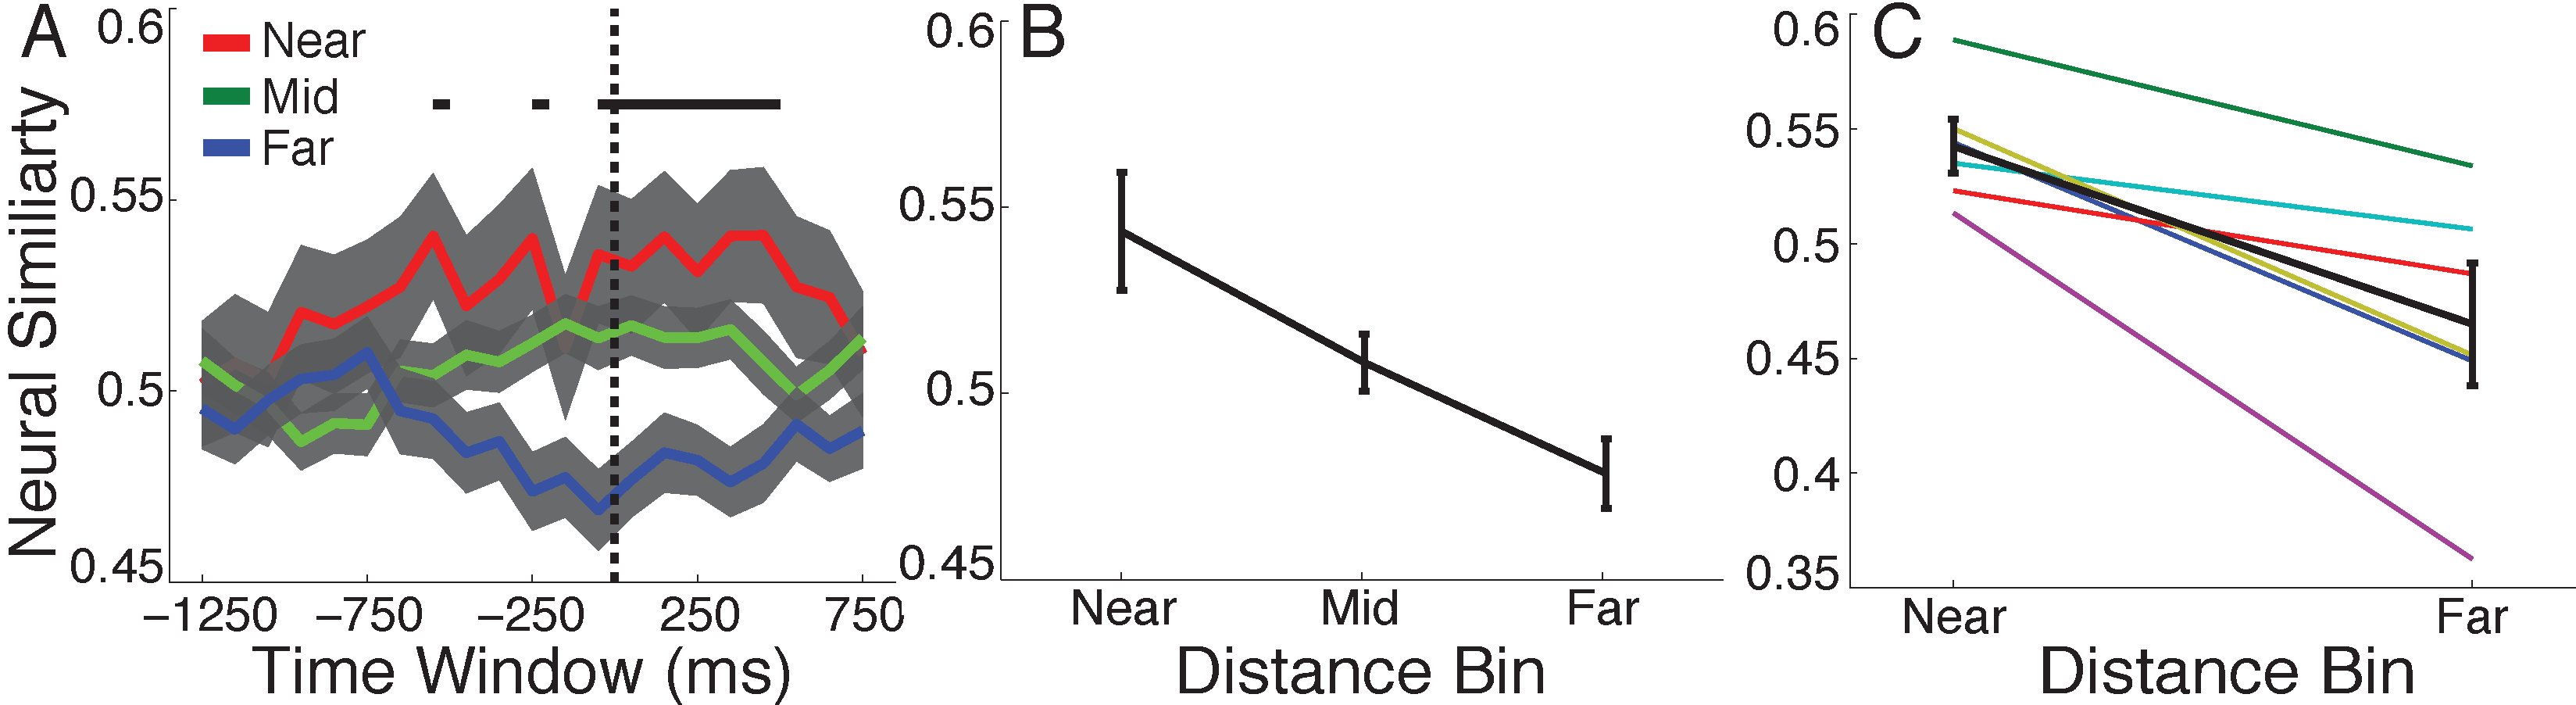
\includegraphics[width=1\textwidth]{./tex/dboy/figs/fig3}
  \caption[Timecourse of neural similarity]{\textbf{A.} Timecourses of neural similarity between ensemble place cell activity during navigation and during item recall are shown for near, middle, and far spatial distance bins.  Timecourses, shown relative to recall onset, were  computed in overlapping 500-ms windows (x-values indicate the center of the window).  Similarity is defined as the cosine of the angle between ensemble activity during recall and navigation, normalized as a rank score. Shaded regions indicate standard error of the mean across recalled items. The horizontal bar indicates significant timepoints as determined by an ANOVA with a false discovery rate adjusted significance threshold of 0.017.  \textbf{B.} The average neural similarity for near, middle, and far spatial distance bins are shown for the time period -300--700 ms relative to recall onset. Error bars indicate standard error of the mean across recalled items.  \textbf{C.} The neural similarity for near and far spatial distance bins for each of the included subjects (thin colored lines) and the subject average (thick black line) are shown for the  time period -300--700 ms relative to recall onset. Error bars indicate standard error of the mean across subjects.}
\label{fig:reinstate}
\end{figure}

During the spontaneous recall of an item, place-responsive cells exhibited firing patterns similar to those they showed during exploration of the region of the town where the item was previously delivered.  Thus, recalling an episodic memory involves recovery of its spatial context, as seen in the activity of place-responsive cells in the human hippocampal formation and surrounding MTL regions. If the object delivery occurred in or near a cell's place field, characterized by a significantly higher than baseline firing rate, then recalling the object should also produce an increase in firing rate. We calculated the firing rate of place-responsive cells when subjects were navigating inside and outside of each cell's place field, as well as the firing rate when subjects recalled items that were presented near to or far from each cell's respective place field (Fig.~\ref{fig:fr_by_cond}) (see Fig.~\ref{fig:fr_by_cond_methods} for further details).  The average in-field firing rate (3.8 Hz) was substantially higher than the out-of-field firing rate  (1.9 Hz; $t$(32) = 5.9, $p < 10^{-5}$).  The average firing rate during the recall of items presented near a place field was 2.2 Hz, which was significantly higher than the 1.8 Hz firing rate during recall of items presented far from a place field ($t$(32) = 2.2, $p =$ .03).

% \section{Discussion?}

Unlike traditional list recall studies of episodic memory, where items unfold only in time, the present experiment provided a unique spatial context for each item.  This allowed us to leverage the  spatial-coding properties of hippocampal neurons in the study of the neural basis of episodic recollection.  Spatially-sensitive neural activity in the hippocampal formation became reactivated during episodic retrieval, when no visual cues were present.  At the time of recall, subjects simply vocalized the names of the delivered objects in the order they came to mind, yet the neurons responsive to spatial  information reactivated during the time just before and during vocalization.  This reactivation implies  that  each experienced item is bound to its spatial context, which in turn may be reinstated when the item comes to mind during recall.  

\begin{figure}
\centering
  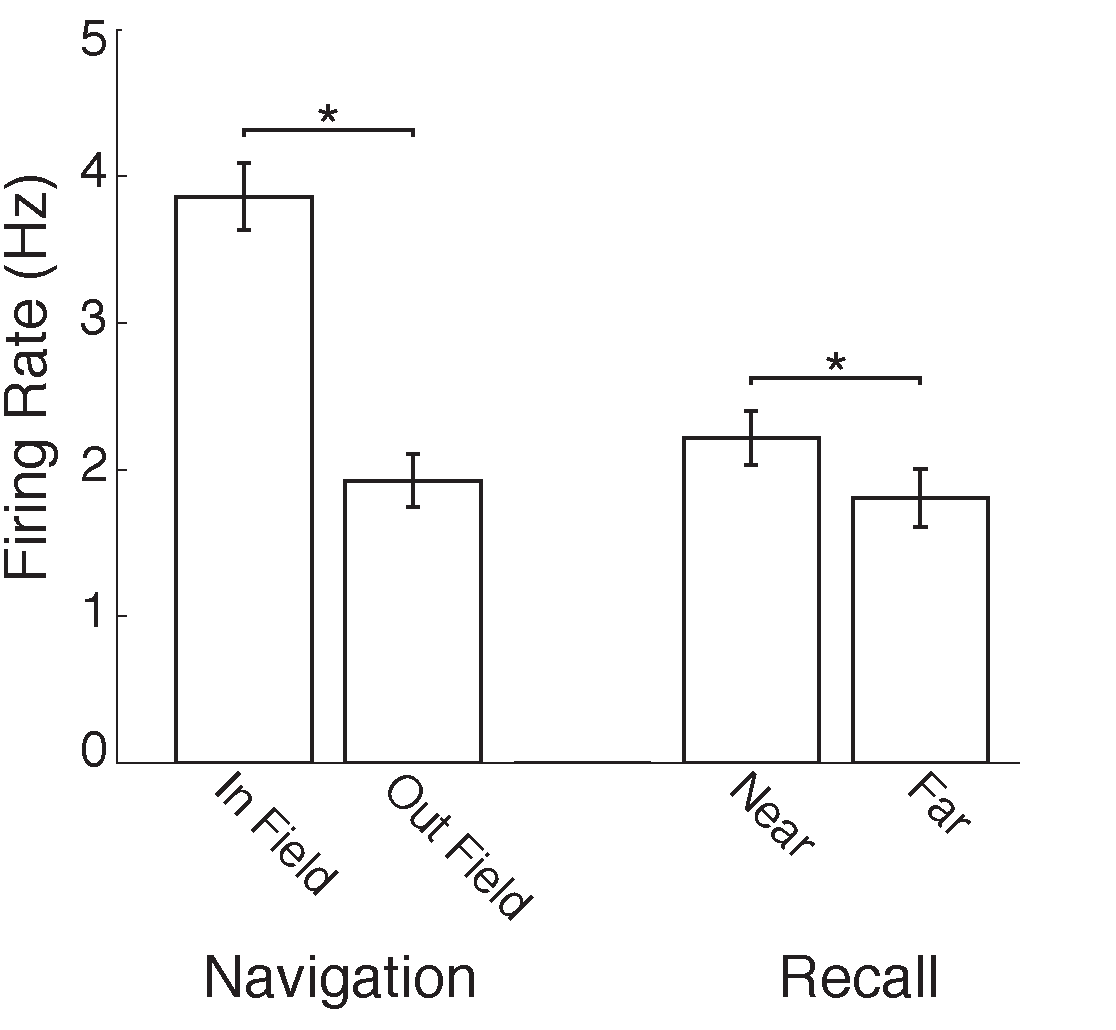
\includegraphics[width=.6\textwidth]{./tex/dboy/figs/fig4}
  \caption[Place-responsive cell firing rate by condition]{Place-responsive cell firing rate by condition. \textbf{Navigation.} In Field indicates the average place-responsive cell firing rate when navigating within a cell's place field, whereas Out Field indicates the average place-responsive cell firing rate at locations outside of a place field ($p < 10^{-5}$). \textbf{Recall.} Near indicates the average place-responsive cell firing rate in time period -1.5 s before to 1 s after recall onset of items that were initially presented in or close to the center of a place field, and, in contrast, Far represents the average place-responsive cell firing rate in the same time window for recall of items that were initially presented far from the center of a place field ($p =$ .03).}
\label{fig:fr_by_cond}
\end{figure}

Because human neural recordings are rarely possible, little is known about the neural substrates of spontaneous verbal recall.  Nonetheless, several recent studies have established the general phenomena of content reinstatement, whereby the attributes of an item at encoding become reinstated just prior to recall.  This has been shown for human hippocampal neurons that are selective for taxonomic categories, or possibly individual items \cite{GelbEtal08}, and also for distributed patterns of intracranial EEG and hemodynamic activity \cite{MannEtal12,PolyEtal05}.  Reinstatement is not specific to an individual item but also spills over onto neighboring items as would be expected if those neighboring items provide an abstract temporal context for the recalled item \cite{MannEtal11,HowaEtal12}.  Such a temporal context signal may be reflected in the recent discovery of individual neurons in the rodent hippocampus that appear to encode the relative times of behaviorally significant events \cite{PastEtal08,MacDEtal11}.

Our finding that spontaneous recall of an item reactivates its spatial context provides direct neural evidence for theories of episodic memory that postulate context reinstatement as the basis for recollection~\cite{PolyKaha08,PolyEtal09}.  It also argues that the spatial coding identified with  the hippocampal place cell system is part of a more general engine of episodic memory in which items become associated with their spatiotemporal contexts and retrieval of items reinstates those contexts to help cue other context-appropriate memories.


\section{Supplemental Materials and Methods}

Seven patients volunteered to participate in this research protocol, which was approved by the institutional review boards at both the University Clinic in Freiburg, Germany, and the University of Pennsylvania.  The patients participated in a total of 65 delivery days spread across 16 experimental sessions each lasting approximately 1 hr.   Across these sessions, we successfully isolated a total of 371 putative neurons from microelectrode recordings in the MTL.  Among these 371 units, 189 were from the hippocampus, 72 were from the entorhinal cortex, 59 were from the amygdala, 20 were from the parahippocampal gyrus, and 31 were localized to the anterior MTL, but not a specific subregion (Table \ref{tab:counts}). See ``Data Acquisition'' below for a further description of localization methods.  A small number of units recorded outside of these MTL regions are excluded from subsequent analyses.

\subsection*{``Delivery Person'' Task}

Subjects performed a hybrid spatial navigation---episodic memory task in which they played the role of a delivery person, delivering objects to stores in a virtual town.  The task consisted of an initial familiarization phase during which subjects learning the locations of all of the stores in the virtual town, followed by a series of ``delivery days''.  On each delivery day, subjects delivered a set of pseudorandomly chosen objects to a subset of the stores and then the screen went blank and they were instructed to recall as many of the delivered objects as they could remember in any order.  In this sense, each delivery day was analogous to a study-test trial of a traditional free recall task.

The virtual town was made up of 16 unique stores (chosen randomly from a pool of 22 stores) and 42 buildings, along with trees, benches, mailboxes, street lights, and areas of grass.  Though the subset of stores chosen at the start of a session differed, the layout of the town was constant. Each store was modeled with a distinct storefront and unique visual features, allowing them to be easily recognizable.  Subjects navigated the environment using a game controller to modulate direction of movement with movement being restricted to roads.  The 3d models used in the virtual environment were created using Autodesk Maya$^{TM}$. The environment was displayed to subjects using the Panda Experiment Programming Library~\cite{SolwEtal13}, which is an in-house Python based wrapper around Panda3d, an open source game engine.

During the familiarization phase at the  start of a session, subjects  were instructed to navigate to each of the 16 stores twice, in a randomly determined order. The current target store was indicated via a text overlay at the top right of the screen (i.e., ``Bitte finden Sie die B\"{a}ckerei'', which translates as ``Please find the bakery''). After completing the familiarization phase, subjects began a series of delivery days, during which a text overlay instructed the subject to locate a specific store. Upon arrival at the store, a common object was presented.  For subjects 1-5, the image of an object, randomly drawn from a pool of 208 distinct object images, appeared for 2 seconds. Because this version of the task was fairly challenging for subjects, we modified the procedure to use objects that were thematically related to stores.  For subjects 6-7, objects were  chosen from a pool of 420 objects that were thematically related to the stores (approximately 20 possible objects could be delivered to a given store). The names of these objects were previously recorded by a female speaker with clear diction and presented auditorally by the computer during the game.  This change from visual to auditory object presentation was made so that the subjects would hear the object name while viewing the store.  Presented objects could not be repeated within an experimental session. Each delivery can be thought of as an item presentation in a list learning experiment.  After the object presentation, the text overlay instructed subjects to locate a different store. Subjects traveled to 13 randomly selected stores in the town (target stores did not repeat within a single delivery day).  Objects were presented at the first 12 stores, and upon arrival at the 13th store, the screen went blank, a row of asterisks appeared on the screen, and a tone sounded, which signaled the start of the free recall period.  Subjects were given 90 seconds to attempt to recall any of the just delivered items, in any order.  Subjects completed between 1 and 10 delivery days in a single recording session, depending on subject time constrains and willingness.

\subsection*{Data Acquisition}
Recording electrodes were placed in target regions selected on purely clinical grounds. Three to six Behnke-Fried electrodes per patient were stereotactically inserted into medial temporal and neocortical structures. Each Behnke-Fried electrode contained 9 platinum-iridium microwires with a diameter of 40 $\mu$m extending a few millimeter into the tissue at the tip of the electrode. Eight microwires, insulated except for the tip, were used for recording, while the 9th microwire was uninsulated and used as a reference. Electrodes were localized post-operatively on 3D MP-RAGE MRI. Precise neuroanatomic regions were determined using post-implant MRIs. Three neuroradiologists independently evaluated the positions of the electrodes. An electrode was labeled as being in a given region (hippocampus, amygdala, entorhinal cortex, parahippocampal gyrus) if at least two of the three localizations were in agreement. Electrodes for which there was disagreement among the localizations were grouped according to their position in the antero-posterior axis and labeled as either anterior or posterior. To eliminate any possibility of bias, the doctors performed the localizations using only unlabeled brain images, and thus were unaware of the type of neuronal activity observed from each electrode.


Signals from the microwires were recorded with three to six 8-channel amplifiers at a 20kHz sampling rate  with an AD-converter resolution of 16 bits. The signal was low-pass filtered at 5 kHz and high-pass filtered at 0.02 Hz using built-in hardware filters. NeuroExplorer software was used for data acquisition and storage.  Continuous recordings were started on the day of surgery or the 1st postoperative day and lasted for 5-10 days with 2-4 interruptions for clinical procedures. Spike detection and sorting was performed using WavClus v. 2.0 \cite{QuirEtal04}, which first detects spikes and then clusters them based on their wavelet coefficients. To avoid contamination between channels, recording channels were excluded if they shared greater than 50\% of their spikes with another channel on the same depth probe.  Single-units with mean firing rates less than 0.1 Hz or greater than 15 Hz (potential interneurons) were excluded from analyses.

\subsection*{Analysis methods}

Behavioral navigation data was discretized into 250 ms epochs, and the subject's average x- and y-coordinate, heading (binned into cardinal directions), and speed within each 250 ms bin was calculated. We excluded navigation epochs during which subjects were not moving from the analyses. Audio recordings of the free recall portions of the task were annotated to identify each spoken word and mark its time of onset and offset within the audio file.  This was done using TotalRecall---an open source software project designed for annotating recall data \cite{SolwEtal10}.

\subsubsection*{Identifying place-responsive cells} Place-responsive cells were identified by using a rank-sum test to locate areas of the virtual environment where the cell exhibited significantly elevated firing (following similar methods as described in \cite{JacoEtal10}). The virtual environment was divided into a 100 $\times$ 100 grid (VR-units). At each location, a one-tailed Wilcoxon rank-sum test compared the firing rates for all navigation epochs within a 10 VR-unit radius (nearby) to the firing rates for all other navigation epochs (far). There must have been at least 20 nearby epochs for a grid location to be included.  

To determine our significance threshold, this procedure was repeated 100 times with time-shifted firing rate values, whereby the firing rate of the cell in each 250 ms epoch was randomly shifted relative to the navigation data. For each time-shifted dataset, we calculated the p-value threshold at which we would observe at least one place field. A place field was defined as a contiguous area of the environment greater than 2\% of the total traversable area where the p-values fell below the given threshold. We then took the fifth percentile of p-value thresholds for the time-shifted data as our significance value for the unshifted data. This procedure fixes the Type 1 error at 5\%.  To test for place-responsive cells that may exhibit direction specific firing, this whole procedure was repeated separately for each cardinal direction. Here, the nearby firing rate for each grid location only included navigation epochs when the subject was traveling in a given cardinal direction, while the far firing rate included epochs irrespective of direction of travel. We labeled a cell a place-responsive cell if a place field was discovered in any of these conditions.  Because most place-responsive cells exhibited a preferred direction, it is possible that some of these cells responded to particular spatial scenes present while traveling in that cardinal direction.  To help rule out this possibility, we carried out a further analysis of view-responsive cells, as described below.  In brief, we did not find significant counts of view-responsive cells in our dataset.

\subsubsection*{Spatial context reinstatement via ensemble activity} 

We excluded sessions with fewer than four place-responsive cells, leaving 12 separate recording sessions from six subjects, with a total of 105 recalled words and 78 place-responsive cells. We tested for spatial-context reinstatement by comparing the similarity of population neuronal responses between memory retrieval and spatial navigation.  First, we characterized the neural representation of location during navigation by calculating the mean firing rate of each place-responsive cell in each location within a 5 $\times$ 7 grid spanning the environment. We then organized this information by computing a series of population ``place vectors'' (one for each grid location), each of which characterized the mean pattern of neuronal activity across the subject's place-responsive cells.  Place vectors were only computed for locations that were traversed at least 10 times.  In calculating the activity of place-responsive cells, we also excluded  epochs in which objects were delivered, as well as a 250 ms buffer surrounding the object deliveries.  This was done to help protect against potential confounds between item and spatial-context reinstatement.

Next, we characterized the place-responsive cell activity during episodic memory retrieval. For each item recall, we created a population ``recall vector'', comprised of the mean firing rate of each place-responsive cell in a time period surrounding item vocalization. In order to ensure that the recall vector corresponded to only one memory retrieval, we did not compute recall vectors for items that were not sufficiently isolated (defined as another vocalization occurring within the preceding 1500 ms or the following 1000 ms), or for the first recall in the retrieval period.  Next, we measured the degree to which recalling an item involves the reinstatement of the neural pattern that represented the location in the environment where the item was encountered.  To quantify this spatial-context reinstatement, we calculated the cosine similarity between each recall vector and each of the place vectors.  For each recall vector, we then ranked the grid locations based on the similarity of the recall vector with grid locations' associated place vectors (that is, the grid location whose place vector has the highest similarity to the recall vector received a rank of 1).  The rank-order transformation of cosine similarities helps to reduce variability from overall shifts in ensemble navigation-retrieval similarity, which would add noise to our analyses.

The context-reinstatement hypothesis predicts that for a given recall vector, place vectors from locations near the position where the item was encountered would have a higher level of similarity compared to the similarity to place vectors representing locations far from the item's delivery location.  We tested this by, for each recall vector, binning the place vectors into three groups based on euclidean distance to the item's delivery location (near: less than 2, middle: greater than or equal to 2 and less than 4, or far: greater than 4). We then computed the mean rank of the place vectors in each group.  We tested for significant spatial-context reinstatement across all item recalls by using an ANOVA to test for a significant difference in similarity between place vectors from different distance bins. See Fig.~\ref{fig:methods} for a graphical representation of this analysis.

To determine the time period relative to recall onset that exhibited significant reinstatement of place-responsive cell activity, the calculation of recall vectors, similarity scores, and significance values was repeated for twenty-one 500 ms overlapping time windows, beginning 1500 ms prior to recall onset and incremented by 100 ms until 500 ms post item onset (results shown in Fig.~\ref{fig:reinstate}A of the main text).  The resulting p-values were corrected using a False Discovery Rate (FDR) set at 0.05 to control for multiple comparisons \cite{BenjHoch95}. Based on the results of this analysis, one set of recall vectors, one set of similarity scores, and the significance value were recalculated within the largest consecutive block of significant time windows (time windows beginning -300 ms through to 200 ms, thus the 1000 ms period of -300 ms through 700 ms; results shown in Fig.~\ref{fig:reinstate}B of the main text).

We also determined whether the spatial reinstatement effect was present when first computing mean similarity scores within each subject, using the same -300 ms to 700 ms time window as above (results shown in Fig.~\ref{fig:reinstate}C of the main text). Instead of averaging across all recalls, we averaged each subject's near and far similarity scores to obtain subject specific measures. Data from subjects with multiple sessions were first concatenated. A t-test compared the distribution of near similarity scores to far similarity scores.

\subsubsection*{Spatial context reinstatement via individual cell firing rate}
Using the same subset of sessions as in the previous ensemble reinstatement analyses, we performed a separate analysis comparing the firing rate of each place-responsive cell during the recall of items initially presented near a place field to the recall of items initially presented far from a place field.  We first calculated the firing rate of each place-responsive cell when subjects were navigating inside and outside of a cell's place field. As above, place fields were defined as a contiguous area greater than 2\% of the traversable environment for which the significance values fell below the computed threshold (based on the described permutation procedure).  If a cell exhibited a place field in more than one cardinal direction, the mean of the in-field and out-field firing rates for all included directions was calculated.

Next, for each cell and for all included recalled items, we determined if each recalled item was initially presented close to or far from the cell's place field. Here, near is defined as having been presented within a radius equal to the length of the place field's major axis, extending from the field's center of mass, and far is defined as having been presented outside of a radius equal to twice the place field's major axis, extending from field's center of mass (see Fig.~\ref{fig:fr_by_cond_methods} for a graphical representation of the division of the virtual environment). Then, we calculated the average firing rate of the cell within a window beginning 1.5 seconds before and extending 1 second post recall onset. Only cells that contributed data to both conditions were included in the analysis, limiting the number from 78 to 33 cells (for instance, not every cell had a set of recalled items that included initial presentations both near to and far from the place field).

\subsubsection*{Identifying view-responsive cells}
In a previous study of  place-responsive cells during human virtual navigation, \cite{EkstEtal03} identified view cells that were predominantly found in the parahippocmapal region.  Because place and view information can be correlated, we carried out an analysis of view cells to determine whether our finding of spatial context reinstatement was likely to have been driven by view rather than place-cell activity.  We first divided the environment into 22 discrete location and direction dependent regions defined by the presence and visibility of specific landmarks, following the analysis framework outlined in \cite{EkstEtal03}. As stores were the most salient objects in the environment, regions of the environment in which a specific store was clearly visible were treated as a single region, reducing the overall number of regions to 17. We also defined regions  in which no specific store was visible but which contained consistent views (for example, of a tall apartment building; see Fig.~\ref{fig:view_methods} for a schematic of the binning of the environment).  Only epochs of movement in which the direction of travel (heading) was within 15 degrees of parallel to the corresponding region were included (this was to ensure consistency of view information).  Then, for each cell, we performed a one-way ANOVA of the firing rate with region as the grouping variable (regions with less than 20 observations were excluded). We next repeated the analysis 100 times with time-shifted firing rate values, in which the firing rate of the cell in each 250 ms epoch was randomly shifted relative to the navigation data.  To be labeled a view-responsive cell, we required that the true ANOVA p-value (calculated on the unshifted data) was less than the 5\% percentile in the distribution of p-values found using the time-shifted data.  Results of this analysis are reported in the supplemental text, below.  To determine if these view-responsive cells could be responsible for the reinstatement effects, we reran the reinstatement analyses, excluding any place-responsive cells that were also labeled as view-responsive. For the spatial context reinstatement via ensemble activity analysis, we used the previously identified -300 ms through 700 ms time interval.  Results of this analysis are reported in the supplemental text, below.

\subsubsection*{Spatial clustering of recalls analysis}

We calculated a spatial clustering score to determine whether our subjects, on aggregate, exhibited knowledge of the locations of the delivered objects. The spatial clustering score is a measure of the tendency for items delivered to spatially proximate locations to be recalled consecutively during the retrieval period \cite{MillEtal12a}. To calculate this score, for each trial, every transition between a recalled item and the following item is ranked based on the distance between their delivery locations. If the Euclidean distance between the delivery locations of two consecutively recalled items is the shortest of all the possible distances, that transition will be giving a score of 1 (conversely, if it is the longest, it will be given a score of 0). For each trial, we calculated an average score, and then we averaged across all 65 trials in our dataset. To calculate the significance level of this score, we repeated this procedure 1000 times, each time randomly permuting the order of the recalled items (while maintaining the same recalled items). This randomization procedure disrupts any spatial clustering that may be present in the recall sequence beyond what would be expected by chance given the subset of recalled items. We then calculated a p-value by seeing where in this distribution the true spatial clustering score lies.

\subsubsection*{View-responsive cells}
We identified 18 view-responsive cells, which was below the Type-I error rate of 19. This failure to detect significant numbers of view-responsive cells is perhaps not surprising in light of the fact that we recorded comparatively  few neurons in the parahippocampal region.  Of the 18 view-responsive cells, 8 also met our criteria for place-responsivity.  Although the number of view-responsive cells was not reliably greater than expected by chance, we nonetheless confirmed that our spatial context reinstatement effect was robust to the exclusion of these 8 cells.  Recalculating the effect for the same interval as reported in our main analysis (-300 to 700 ms)  revealed a significant difference between the spatial distance bins both on the level of recalls ($F$(2,297) = 5.6, $p <$ .01) and on the individual participant level ($t$(5) = 3.9, $p =$ .01).  Additionally, we recalculated the distributions of place-responsive cell firing rates during the recall of items initially presented near and far from place fields, excluding any view-responsive cells from the analysis (lowering the number of included cells from 33 to 31). The average firing rate during the recall of items presented near a place field was 2.3 Hz, significantly higher than the 1.9 Hz firing rate during recall of items presented far from a place field ($t$(30) = 2.3, $p =$ .03)

\subsubsection*{Spatial clustering}
The spatial clustering score for our dataset was .54, significantly greater than the chance level determined by the permutation procedure ($p = .008$).  Though our data were too sparse to determine significance of spatial clustering within individual subjects, we note that 6 out of 7 subjects exhibited greater than chance spatial clustering scores.

\clearpage
\section{Supplemental Figures}

 \begin{figure}[ht]
\centering
  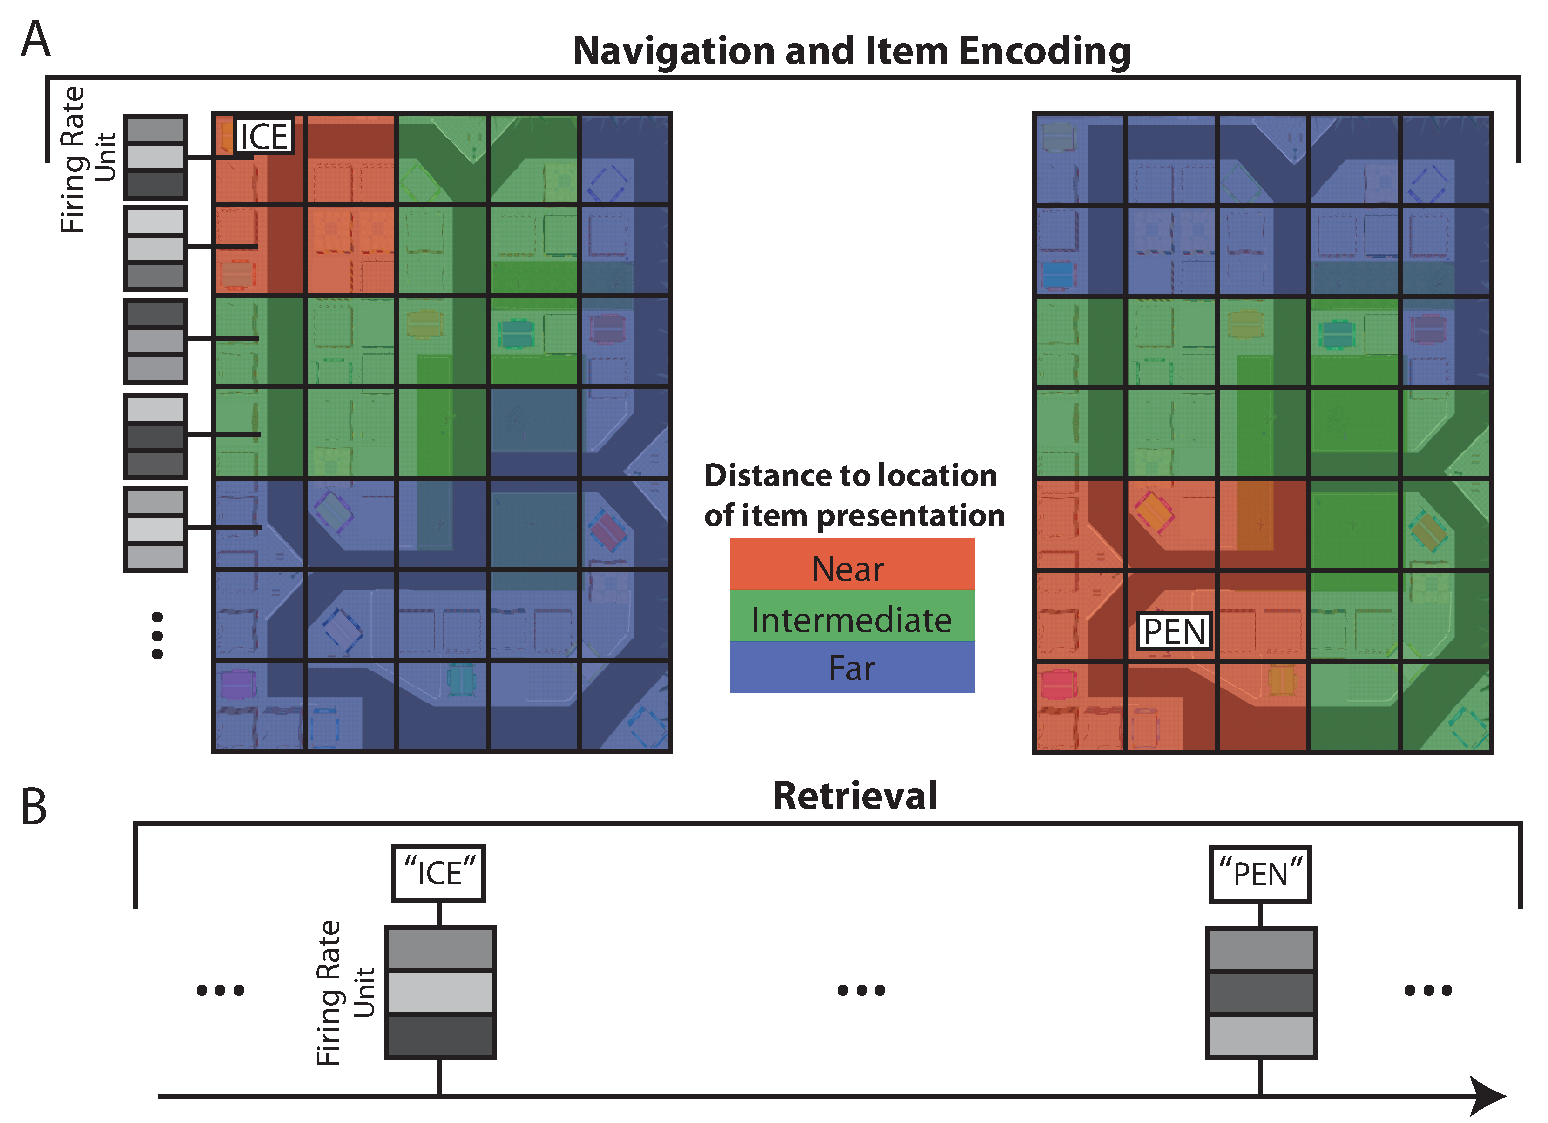
\includegraphics[width=.95\textwidth]{./tex/dboy/figs/methods}
  \caption[Spatial context reinstatement analysis method]{A schematic of the spatial context reinstatement via ensemble activity analysis. In these hypothetical examples, an item is presented to the subject in a particular sector of the town, as indicated in Panel A.  Red shading indicates sectors considered spatially close the presentation location, green shading indicates sectors considered spatially intermediate, and blue shading indicates sectors considered spatially far. In a given session, the mean firing rate of all identified place-responsive cells was calculated separately for each sector (represented visually by the shaded grey boxes).  During retrieval of the same item, the mean activity of the place-responsive cells was calculated.  \textbf{A.} Two examples of the spatial binning of the environment. Left: the spatial binning of the environment if an item (``Ice'') was presented in the location indicated. Right: the spatial binning of the environment if an item (``Pen'') was presented in the location indicated.  \textbf{B.} In the retrieval period, the mean place-responsive cell firing rate during each item recall is calculated and compared the navigation activity (recall of ``Ice'' uses the spatial binning shown in panel A Left and recall of ``Pen'' uses the spatial binning shown in panel A Right).}
\label{fig:methods}
\end{figure}

 \begin{figure}
\centering
  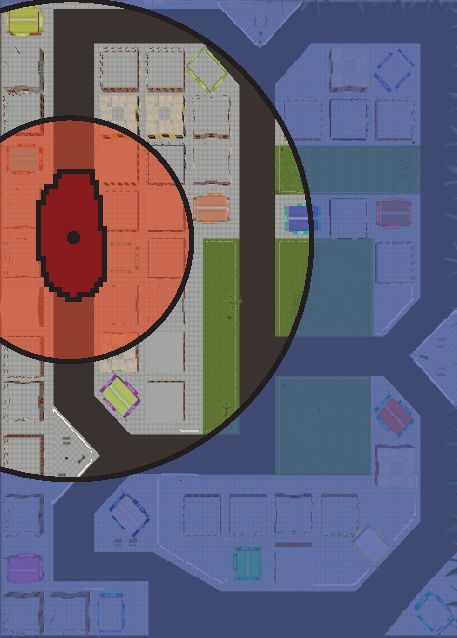
\includegraphics[width=.6\textwidth]{./tex/dboy/figs/firing_rate_method}
  \caption[Spatial context reinstatement via individual cell firing rate analysis method]{A visual representation of the spatial context reinstatement via individual cell firing rate analysis. The dark red area represents a cell's place field, and the dot in the middle of the place field represents the center of mass.  Items delivered to the store falling within the transparent red circle would be considered near to the place field. Items delivered to stores falling within the transparent blue circle would be considered far from the place field. The radii of the circles emanating from the center of mass are determined by the length of the major axis of the place field (1 times the major axis and 2 times the major axis for near and far, respectively).}
\label{fig:fr_by_cond_methods}
\end{figure}

 \begin{figure}
\centering
  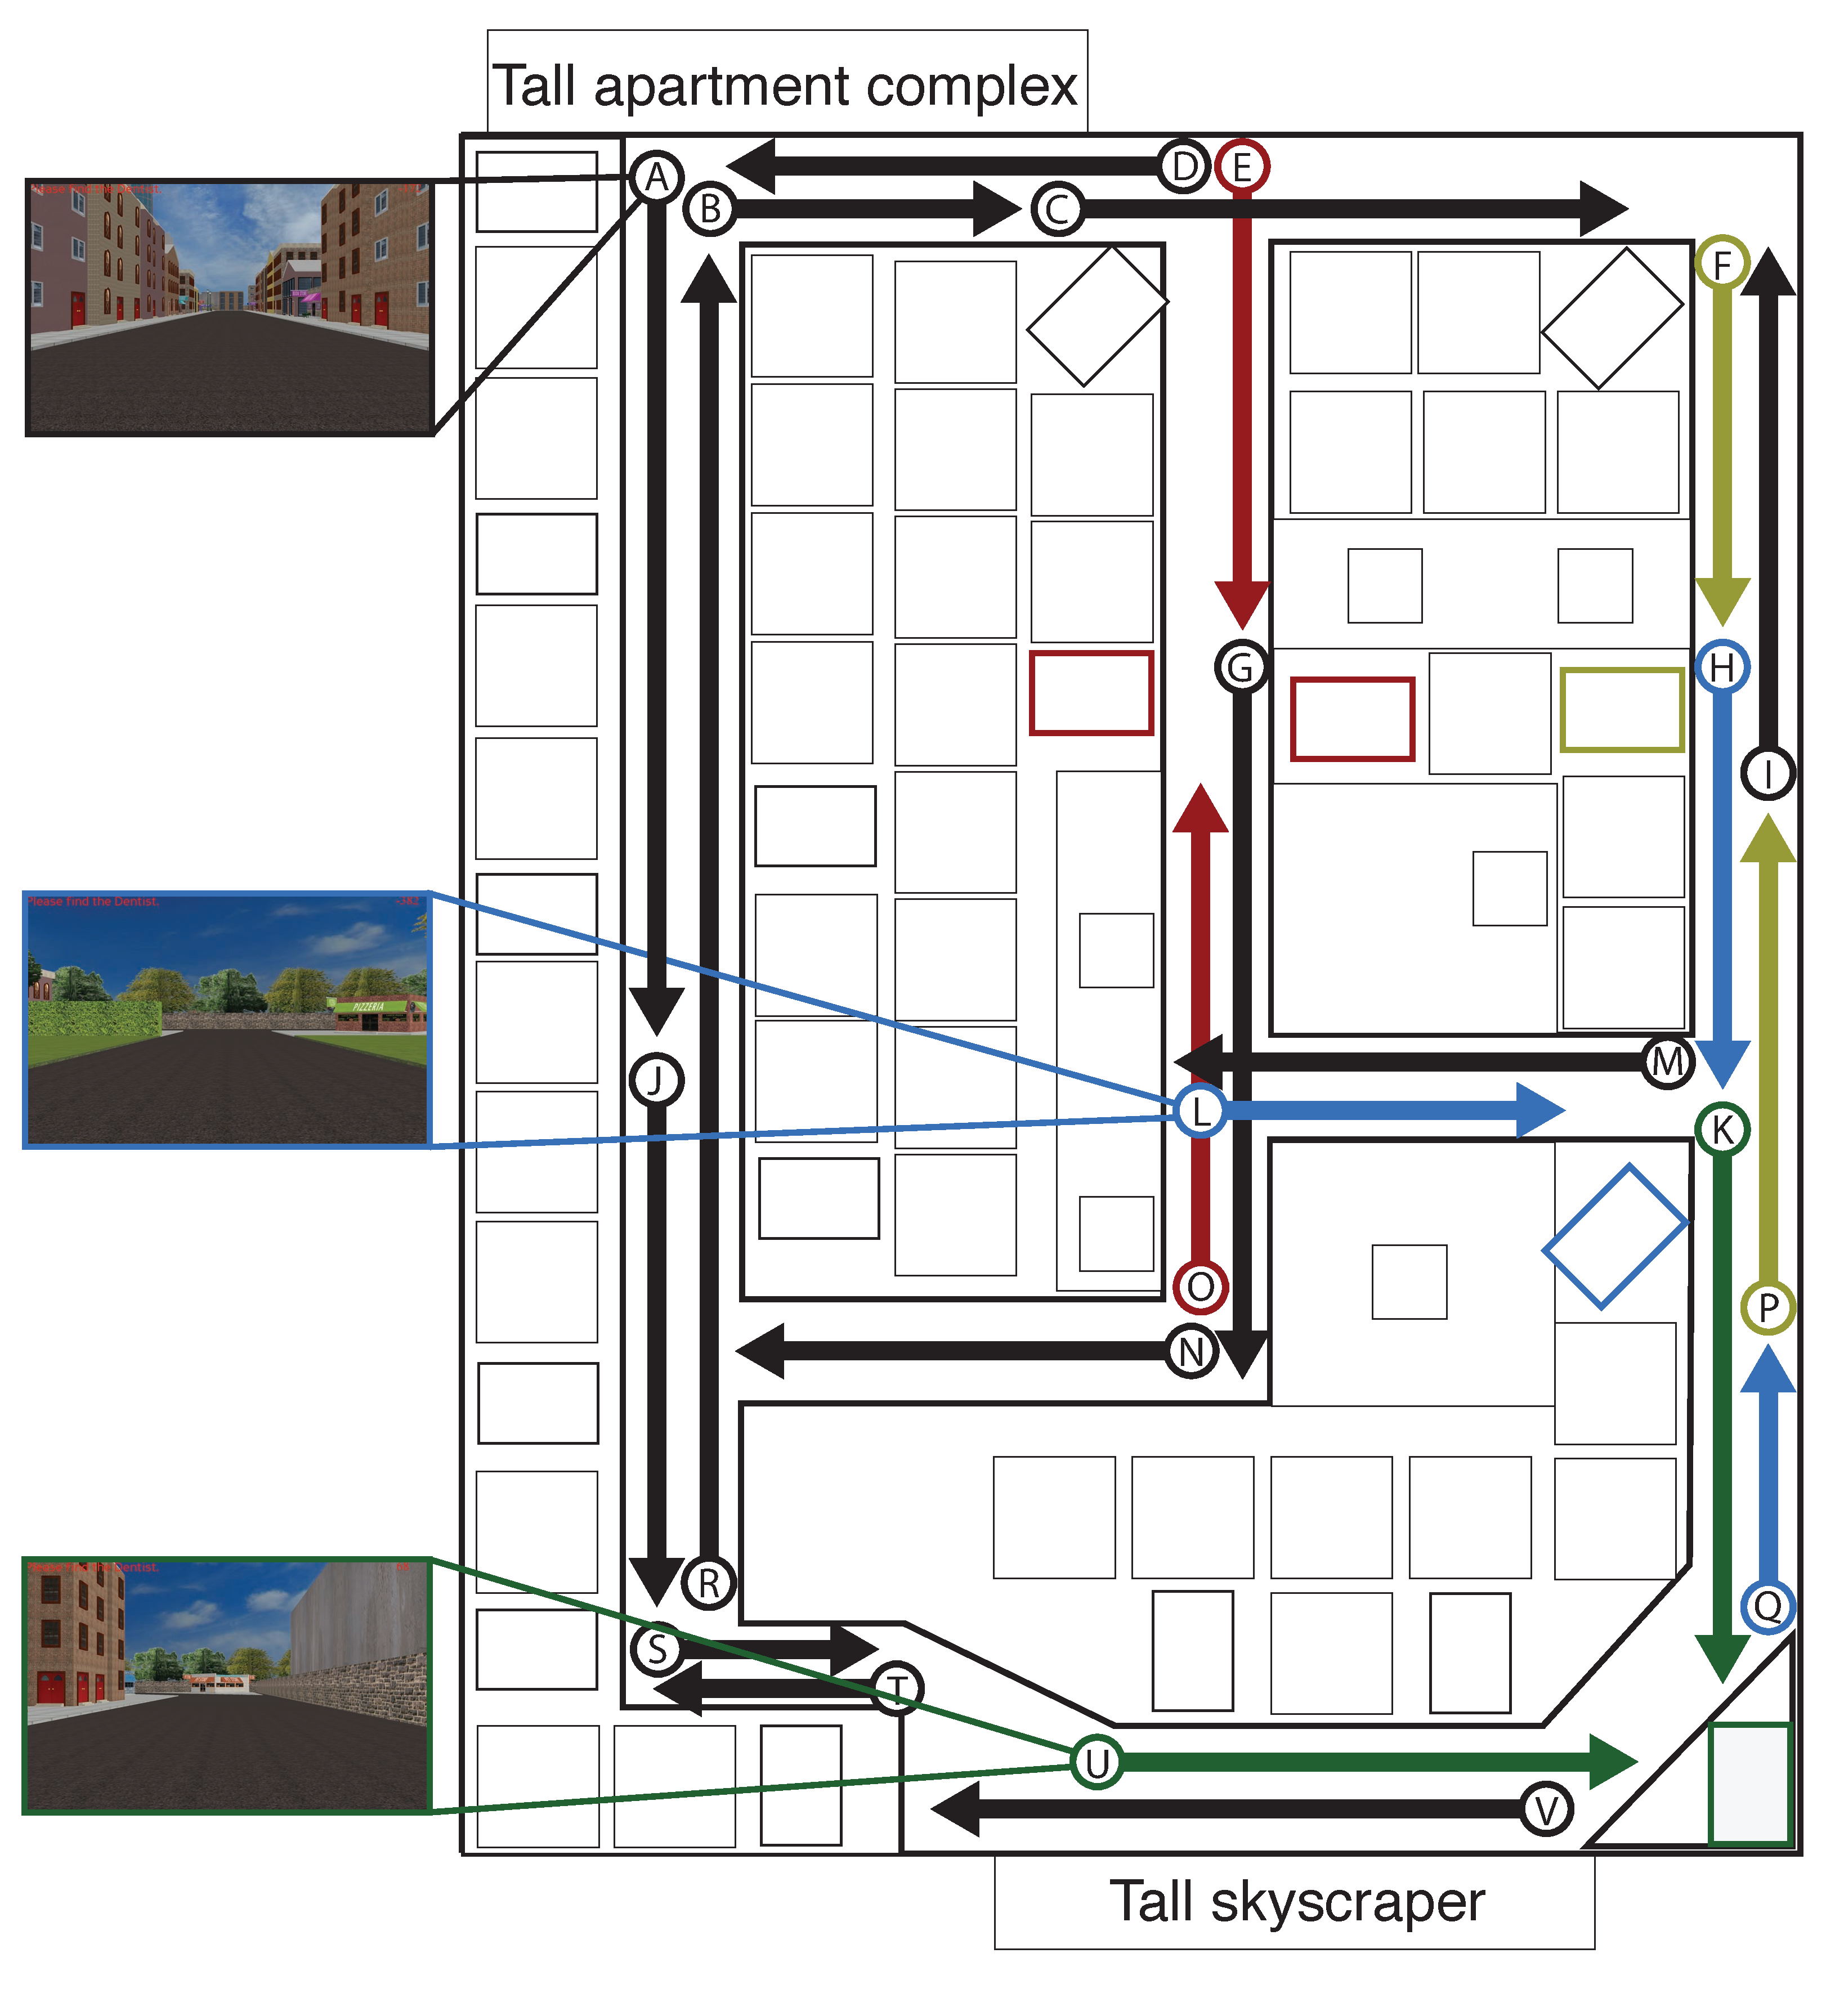
\includegraphics[width=.7\textheight]{./tex/dboy/figs/viewSmall}
  \caption[View-responsive cell analysis method]{A visual representation of how the environment was divided into regions for the view-responsive cell analysis. Each arrow represents the area of the town and direction of travel for its respective region. Arrows with the same color (excluding black arrows, which are all distinct regions) shared a primary landmark, and thus were treated in the analysis as the same region (colored rectangles represent the landmark shared among these regions). For illustrative purposes, screenshots of three of the regions are shown on the left (regions \emph{A}, \emph{L}, and \emph{U}, taken at the beginning (tail end) of their respective arrows. Note that the field of view during navigation was 60$^\circ$, thus objects and landmarks immediately to sides of the current location are not visible.}
\label{fig:view_methods}
\end{figure}

\clearpage
\section{Supplemental Tables}
\begin{table}[ph]
\centering
%  \begin{scriptsize}
% \begin{tabular}{|c|C{.8cm}|C{1.3cm}|C{1cm}|C{1cm}|C{1cm}|C{.8cm}|C{.8cm}|C{1cm}|C{.8cm}|C{.8cm}|}
 \begin{tabular}{|ccc|ccccc||c|}

\multicolumn{3}{c|}{} & \multicolumn{5}{|c||}{Region} & \multicolumn{1}{c}{}\\\hline
      Subject $\#$ & Session & Trials & H & A & EC & PHG & ANT & Totals\\\hline
      \multirow{3}{*}{1} & 1 & 1 & 4 of 16 & 2 of 5 & 5 of 8 & 0 of 0 & 0 of 0 & 11 of 29\\
      & 2 & 1 & 5 of 26 & 0 of 4 & 5 of 11 & 0 of 0 & 0 of 0 & 10 of 41\\
      & 3 & 2 & 6 of 17 & 0 of 5 & 1 of 8 & 0 of 0 & 0 of 0 & 7 of 30\\\hline
      \multirow{3}{*}{2} & 1 & 1 & 6 of 8 & 0 of 0 & 2 of 9 & 1 of 7 & 0 of 0 & 9 of 24\\
      & 2 & 3 & 0 of 0 & 0 of 0 & 4 of 11 & 0 of 7 & 0 of 0 & 4 of 18\\
      & 3 & 2 & 1 of 4 & 0 of 0 & 1 of 8 & 0 of 6 & 0 of 0 & 2 of 18\\\hline
      \multirow{3}{*}{3} & 1 & 3 & 6 of 17 & 3 of 7 & 0 of 0 & 0 of 0 & 0 of 0 & 9 of 24\\
      & 2 & 3 & 4 of 10 & 1 of 4 & 0 of 0 & 0 of 0 & 0 of 0 & 5 of 14\\
      & 3 & 3 & 7 of 17 & 3 of 8 & 0 of 0 & 0 of 0 & 0 of 0 & 10 of 25\\\hline
      \multirow{2}{*}{4} & 1 & 6 & 1 of 4 & 5 of 9 & 0 of 0 & 0 of 0 & 1 of 4 & 7 of 17\\
      & 2 & 8 & 0 of 1 & 3 of 7 & 0 of 0 & 0 of 0 & 1 of 2 & 4 of 10\\\hline
      5 & 1 & 6 & 1 of 12 & 0 of 8 & 1 of 8 & 0 of 0 & 0 of 0 & 2 of 28\\\hline
      \multirow{2}{*}{6} & 1 & 4 & 1 of 10 & 0 of 2 & 0 of 0 & 0 of 0 & 1 of 14 & 2 of 26\\
      & 2 & 4 & 1 of 13 & 0 of 0 & 0 of 0 & 0 of 0 & 3 of 11 & 4 of 24\\\hline
      \multirow{2}{*}{7}  & 1 & 10 & 1 of 17 & 0 of 0 & 3 of 7 & 0 of 0 & 0 of 0 & 4 of 24\\
      & 2 & 8 & 4 of 17 & 0 of 0 & 1 of 2 & 0 of 0 & 0 of 0 & 5 of 19\\
\hline
\multicolumn{3}{c|}{Totals} & 48 of 189 & 17 of 59 & 23 of 72 & 1 of 20 & 6 of 31 & \multicolumn{1}{c}{95 of 371}\\
    \end{tabular}
%  \end{scriptsize}
  \caption[Summary of place-responsive cells]{Summary of place-responsive cell counts across subjects. The table shows the total number of cells and the total number of place-responsive cells for each recording session, aggregated by brain region (H: hippocampus, A: amygdala, EC: entorhinal cortex, PHG: parahippocampal gyrus, ANT: localization accuracy limited to anterior MTL). Sessions with less than four place-responsive cells were excluded from reinstatement analyses. Though session 1 of subject 1 had 11 identified place-responsive cells, it was excluded from the reinstatement analyses due to not having any valid recalls.}
\label{tab:counts}
\end{table}

\clearpage



\begin{table}[ph]
\centering
%  \begin{scriptsize}
% \begin{tabular}{|c|C{.8cm}|C{1.3cm}|C{1cm}|C{1cm}|C{1cm}|C{.8cm}|C{.8cm}|C{1cm}|C{.8cm}|C{.8cm}|}
 \begin{tabular}{|c|lcccc|}
\hline
Subject $\#$ & Region & $\#$ Cells & FR (Hz) & In Field FR (Hz) & Field Size\\\hline

\multirow{4}{*}{1} & Amygdala & 2 of 14  & 0.18 & 0.54 & 2.64 \\ 
 & EC & 11 of 27  & 2.09 & 3.60 & 2.59 \\ 
 & Hipp Body & 8 of 31  & 0.82 & 2.94 & 2.76 \\ 
 & Hipp Head & 7 of 28  & 0.32 & 0.89 & 2.77 \\ \hline
\multirow{3}{*}{2} & EC & 7 of 28  & 1.82 & 4.53 & 2.68 \\ 
 & Hipp Body & 7 of 12  & 0.37 & 5.97 & 3.26 \\ 
 & PHG & 1 of 20  & 0.39 & 4.48 & 5.43 \\ \hline
\multirow{2}{*}{3} & Amygdala & 7 of 19  & 0.63 & 2.38 & 2.47 \\ 
 & Hipp Head & 17 of 44  & 1.28 & 2.62 & 2.41 \\ \hline
\multirow{3}{*}{4} & Amygdala & 8 of 16  & 4.07 & 5.64 & 2.43 \\ 
 & Hipp Head & 1 of 5  & 0.23 & 0.82 & 2.37 \\ 
 & Anterior MTL & 2 of 6  & 0.35 & 1.22 & 2.46 \\ \hline
\multirow{3}{*}{5} & Amygdala & 0 of 8  & - & - & - \\ 
 & EC & 1 of 8  & 0.05 & 0.60 & 2.35 \\ 
 & Hipp Head & 1 of 12  & 0.27 & 1.12 & 2.20 \\ \hline
\multirow{4}{*}{6} & Amygdala & 0 of 2  & - & - & - \\  
 & Hipp Head & 2 of 15  & 0.15 & 1.60 & 3.01 \\ 
 & Hipp Tail & 0 of 8  & - & - & - \\ 
 & Anterior MTL & 4 of 25  & 7.78 & 9.71 & 2.52 \\ \hline
\multirow{3}{*}{7} & EC & 4 of 9  & 1.31 & 2.32 & 2.90 \\ 
 & Hipp Body & 4 of 21  & 6.13 & 7.87 & 2.52 \\ 
 & Hipp Head & 1 of 13  & 3.89 & 5.38 & 2.37 \\ 
\hline
    \end{tabular}
%  \end{scriptsize}
  \caption[Place-responsive cells characteristics]{Place-responsive cells characteristics by subject and region. For each subject, only regions in which cells were recorded are included. The column ``$\#$ Cells'' shows the number of place-responsive cells recorded, out of the total number of cells. The column ``FR (Hz)'' shows the average firing rate within a region  for all movement epochs during the task, regardless of location in the virtual environment.  The column ``In Field FR (Hz)'' shows the average firing rate within a region within the cells' place fields. The column ``Field Size'' shows the average size of the place fields within a region as a percentage of the traversable area of the virtual environment.}
\label{tab:counts2}
\end{table}




\clearpage

% \bibliographystyle{Science}

